\documentclass[a4paper]{article}

\usepackage[english]{babel}
\usepackage[utf8]{inputenc}
\usepackage{fullpage}
\usepackage{multicol}
\usepackage{graphicx}
\usepackage{caption}

\newenvironment{Figure}
  {\par\medskip\noindent\minipage{\linewidth}}
  {\endminipage\par\medskip}

% \title{(Dynamic) Neural Network Modules}
% \author{Matěj Nikl}
% \date{}

% \pagenumbering{gobble}

\begin{document}

\begin{multicols}{2}
\section*{(Dynamic) Neural Network Modules}

This paper tries to address the task of (visual) question answering. One might try to approach this problem with a single, monolithic, deep NN, which would somehow try to answer all possible questions about all possible images (or \textit{worlds} as they are called in general). Authors of this paper, however, tried to tackle this problem in a different way. Take for example a question ``What si in the sheep's ear?''. It can be broken down into smaller subtasks/processing steps:
\begin{enumerate}
    \item find sheeps
    \item find ears
    \item \textit{intersect} those two locations
    \item describe what is in the intersection
\end{enumerate}

Those subtasks arise in every question because of the compositional nature of language.

\begin{Figure}
    \centering
    \frame{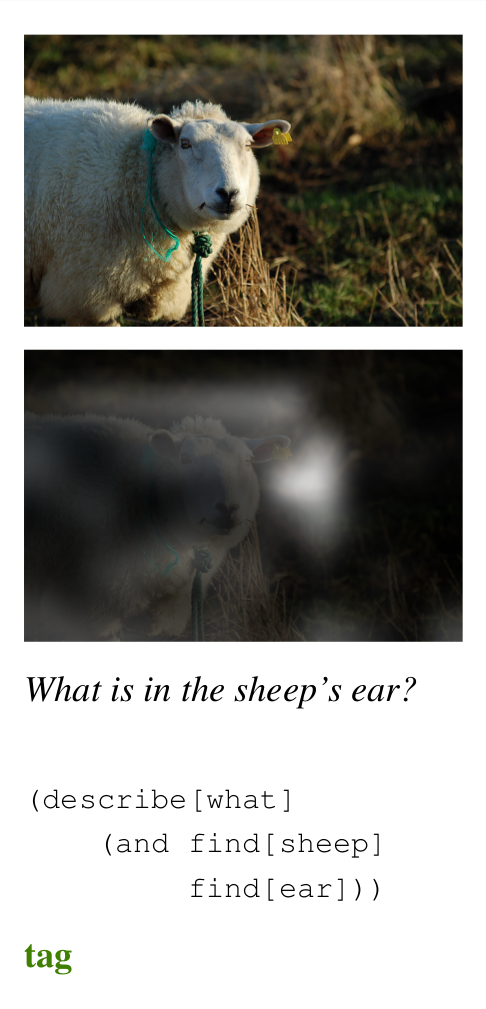
\includegraphics[width=0.48\textwidth]{sheep.png}}
    \frame{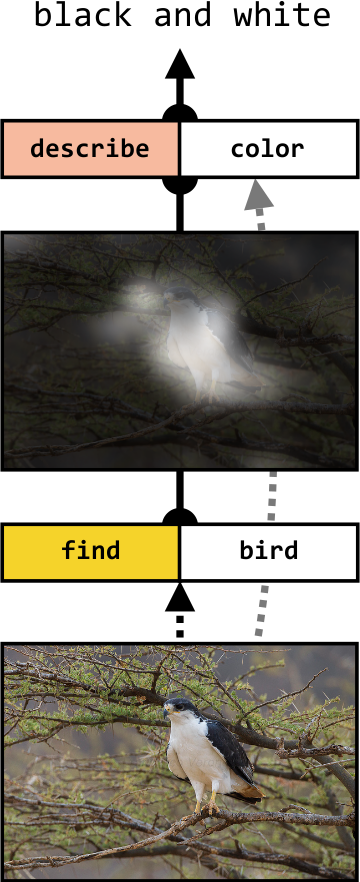
\includegraphics[width=0.48\textwidth]{bird.png}}
    \captionof{figure}{examples of network instances and their computations}
\end{Figure}

    Applying these operations would lead to the correct answer. Thus, it was proposed to use such modules that would compute those simpler operations and compose them for each question in a way that would lead to a correct answer being produced. This gives a rise to a few more problems to solve. What types of modules do we need to sufficiently express any question given? How these modules should be designed, how will they communicate and how will we train them? And finally, how to determine how to arrange those modules into a network so that it would answer the question given?

This is the minimal set of modules described in the paper:
\begin{itemize}
    \item Lookup
    \item Find$[x]$ – finds/locates $x$ and produces attention map
    \item Relate – similiar to find, also takes in account current region of attention
    \item And – perform a \textit{intersect} operation on attention maps
    \item Describe – predicts an answer representation from attention map
    \item Exists
\end{itemize}

They all have their own purposes and might be useful on their own, however their true
power comes when they get arranged to form a tree of operations, applying one after another, performing potentially more complex computation at each step.

\subsection*{Assembling modules into networks}
    The proposed approach is to perform a syntactic parse on the question to generate a small set of layout candidates. To choose the best one, all layouts need to be scored. For that a LSTM representation of the question, as well as a feature-based representation of the layout being scored, are produced and passed through a MLP. The layout feature vector includes indicators of the number of modules of each type present and their arguments (e.g. that a find module is looking for a dog).

    As soon as we choose our best layout, we can maximize the log-likelihood of the correct answer being produced (with a standard backpropagation). However, choosing the best layout is nondifferentiable, thus different technique called reinforcement learning must be used.

\end{multicols}
\end{document}
